\chapter{Funções}

\section{Definição de Função}

Dados dois conjuntos $A$ e $B$, não vazios, uma relação $f$ de $A$ em $B$ recebe o nome de aplicação de $A$ em $B$ ou função de $A$ em $B$ se, e somente se, para todo $x \in A$ existe um só $y \in B $ tal que $(x,y) \in f$

\begin{figure}[H]
	\centering
	
	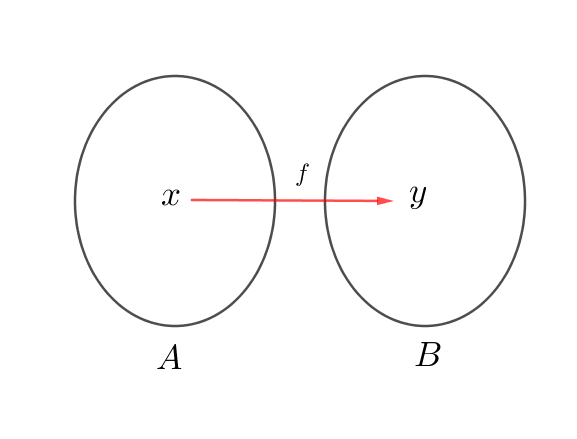
\includegraphics[scale=3.5]{imagens/funcao.png}

\end{figure}

\textbf{Exemplos:}

\begin{enumerate}

\item Dados os conjuntos $A = \{ -1\,;\,0\,;\,1\,;\,2\}$ e $B = \{0\,;\,1\,;\,2\,;\,3\}$, seja a relação $f$ de $A$ em $B$ expressa por $y=x+1$, com $x\in A$ e $y \in B$.

\begin{figure}[H]
	\centering
	
	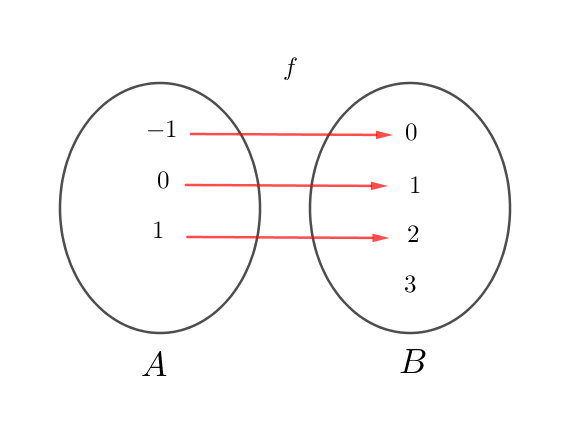
\includegraphics[scale=3.5]{imagens/funcao-ex1.png}

\end{figure}
\begin{itemize}
\item $x= -1 \, \Rightarrow \,y = -1+1 = 0  \, \Rightarrow (-1,0) \in f$
\item $x= 0 \, \Rightarrow \,y = 0+1 = 1 \, \Rightarrow (0,1) \in f $
\item $x= 1 \, \Rightarrow \,y = 1+1 = 2  \, \Rightarrow (1,2) \in f$

\item Todos os elementos de $A$ estão associados a elementos de $B$.
\item A cada elemento de $A$ está associado um único elemento de $B$.
\end{itemize}
Neste caso, a relação $f$ de $A$ em $B$ expressa por $y=x+1$ é uma função de $A$ em $B$.

\item Dados os conjuntos $A = \{ -1\,;\,1\,;\,3\}$ e $B = \{1\,;\,3\,;\,4\,;\,9\}$, seja a relação $f$ de $A$ em $B$ expressa por $y=x^2$, com $x\in A$ e $y \in B$.

\begin{figure}[H]
	\centering
	
	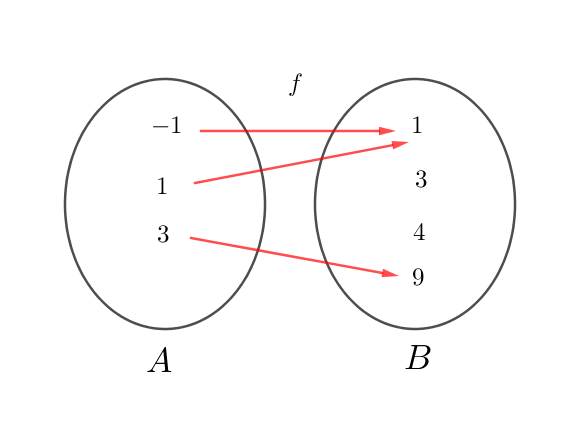
\includegraphics[scale=3.5]{imagens/funcao-ex2.png}

\end{figure}

\begin{itemize}
\item $x= -1 \, \Rightarrow \,y = (-1)^2 = 1 \, \Rightarrow (-1,1) \in f $
\item $x= 1 \, \Rightarrow \,y = (1)^2 = 1  \, \Rightarrow (1,1) \in f$
\item $x= 3 \, \Rightarrow \,y = (3)^2 = 9  \, \Rightarrow (3,9) \in f$

\item Todos os elementos de $A$ estão associados a elementos de $B$.
\item A cada elemento de $A$ está associado um único elemento de $B$.
\end{itemize}
Neste caso, a relação $f$ de $A$ em $B$ expressa por $y=x^2$ é uma função de $A$ em $B$.

\item Dados os conjuntos $A = \{ 0\,;\,1\,;\,2\}$ e $B = \{-1\,;\,0\,;\,1\,;\,4\}$, seja a relação $f$ de $A$ em $B$ expressa por $y^2=x$, com $x\in A$ e $y \in B$.

\begin{figure}[H]
	\centering
	
	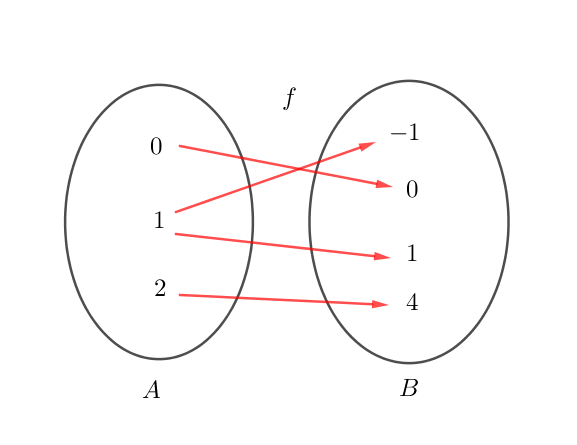
\includegraphics[scale=3.5]{imagens/funcao-ex3.png}

\end{figure}

\begin{itemize}
\item $x= 0 \, \Rightarrow \,y^2 = 0 = 0 \, \Rightarrow (0,0) \in f $
\item $x= 1 \, \Rightarrow \,y^2 = 1 = \pm 1  \, \Rightarrow (1,1)\, \text{e} \, (1,-1)\, \in f$
\item $x= 4 \, \Rightarrow \,y^2 = 4 = 2  \, \Rightarrow (4,2) \in f$

\item Todos os elementos de $A$ estão associados a elementos de $B$.
\item A cada elemento de $A$ \textbf{não} está associado \textbf{um único} elemento de $B$.
\end{itemize}
Neste caso, a relação $f$ de $A$ em $B$ expressa por $y^2=x$ \textbf{não} é uma função de $A$ em $B$.

\end{enumerate}

\section{Domínio, Contradomínio e Imagem de uma Função}

Toda função possui um domínio(digamos que são valores de partida) e uma imagem (valores de chegada).

\begin{figure}[H]
	\centering
	
	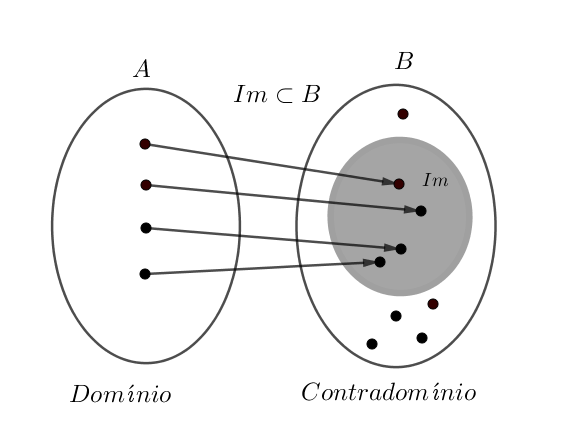
\includegraphics[scale=3.5]{imagens/domi-imag.png}

\end{figure}

\begin{itemize}

\item O domínio de uma função é o conjunto dos elementos de onde as setas partem.

\item A imagem de uma função é o conjunto dos elementos em que as setas chegam.

\item O contradomínio de uma função é o conjunto dos elementos possiveis em que as setas podem chegar.

\end{itemize}
\textbf{Observações:}
\begin{itemize}
\item O conjunto imagem está contido no contradomínio
\item As vezes é possivel que o conjunto imagem seja igual ao contradomínio $Im = B$.
\end{itemize}

\subsection{Pensando em função}

Podemos pensar em uma função como uma máquina. Com $x$ sendo os valores que entram (domínio)  e $y$ sendo os valores de saída (imagem) processados pela máquina. 

\begin{figure}[H]
	\centering
	
	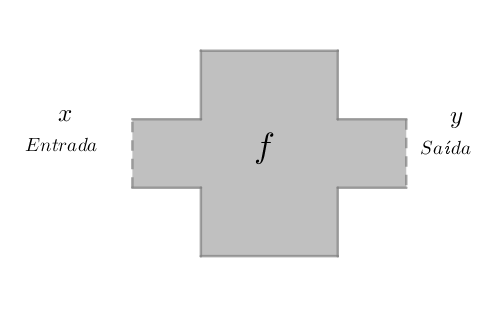
\includegraphics[scale=3.5]{imagens/pensa-funcao.png}

\end{figure}

\section{Gráfico de uma função}

O gráfico de uma função é o conjunto de pares ordenados $(x,y)$ 

\begin{figure}[H]
	\centering
	
	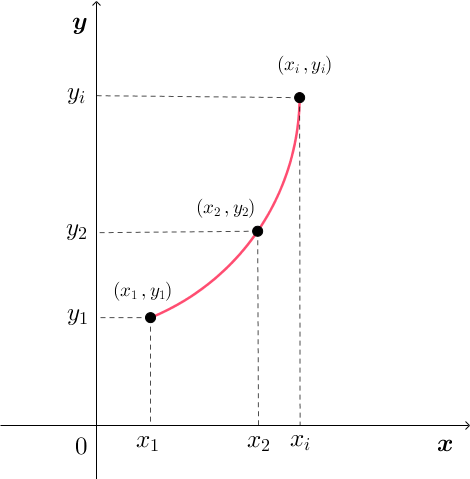
\includegraphics[scale=3.5]{imagens/graf-funcao.png}

\end{figure}